\documentclass[11pt,a4paper]{ctexart}

% ===================== Packages =====================
\usepackage[margin=2.3cm, headheight=23pt]{geometry}
\usepackage{amsmath,amssymb}
\usepackage{graphicx}
\usepackage{booktabs,tabularx,multirow,colortbl}
\usepackage{xcolor}
\usepackage{tikz}
\usetikzlibrary{arrows.meta,positioning,calc}
\usepackage[skins,breakable]{tcolorbox}
\usepackage{float}
\usepackage{enumitem}
\usepackage{fancyhdr}
\usepackage{titlesec}
\usepackage{caption}
\usepackage[unicode=true,colorlinks=true,linkcolor=NavyBlue,urlcolor=RoyalBlue,citecolor=NavyBlue]{hyperref}

% ===================== Colors =====================
\definecolor{NavyBlue}{HTML}{1B365D}
\definecolor{RoyalBlue}{HTML}{2563EB}
\definecolor{SkySoft}{HTML}{EFF6FF}
\definecolor{SlateBg}{HTML}{F8FAFC}
\definecolor{BorderBlue}{HTML}{93C5FD}
\definecolor{AccentTeal}{HTML}{0D9488}
\definecolor{TealSoft}{HTML}{F0FDFA}
\definecolor{AmberSoft}{HTML}{FFFBEB}
\definecolor{AmberBorder}{HTML}{D97706}
\definecolor{Crimson}{HTML}{DC2626}
\definecolor{MutedGray}{HTML}{64748B}
\definecolor{RowGray}{HTML}{F1F5F9}

% ===================== Typography & Layout =====================
\setlength{\parskip}{5pt}
\setlength{\parindent}{0pt}
\renewcommand{\arraystretch}{1.28}
\captionsetup{font={small}, labelfont={bf,color=NavyBlue}, skip=6pt}

\pagestyle{fancy}
\fancyhf{}
\fancyhead[L]{\footnotesize\textcolor{MutedGray}{\textbf{TreeWeave Paper Proposal} $\cdot$ Motivation, Storyline \& Experiments}}
\fancyhead[R]{\footnotesize\textcolor{MutedGray}{Validation Backbone: \texttt{Qwen3.5-4B}}}
\fancyfoot[C]{\footnotesize\textcolor{MutedGray}{\thepage}}
\renewcommand{\headrulewidth}{0.4pt}
\renewcommand{\headrule}{\hbox to\headwidth{\color{BorderBlue}\leaders\hrule height \headrulewidth\hfill}}

\titleformat{\section}
  {\Large\bfseries\color{NavyBlue}}
  {\thesection}{0.6em}{}
  [\vspace{2pt}{\color{BorderBlue}\titlerule[0.8pt]}]

\titleformat{\subsection}
  {\large\bfseries\color{NavyBlue!90!black}}
  {\thesubsection}{0.5em}{}

% ===================== Custom Boxes =====================
\newtcolorbox{insightbox}[1][]{
  enhanced, breakable,
  colback=SkySoft, colframe=RoyalBlue,
  boxrule=0.8pt, left=10pt, right=10pt, top=7pt, bottom=7pt,
  arc=3pt, fonttitle=\bfseries,
  title={#1}
}

\newtcolorbox{storybox}[1][]{
  enhanced, breakable,
  colback=SlateBg, colframe=NavyBlue!75,
  boxrule=0.6pt, left=10pt, right=10pt, top=7pt, bottom=7pt,
  arc=3pt, fonttitle=\bfseries,
  title={#1}
}

\newtcolorbox{claimbox}[1][]{
  enhanced, breakable,
  colback=TealSoft, colframe=AccentTeal,
  boxrule=0.7pt, left=10pt, right=10pt, top=7pt, bottom=7pt,
  arc=3pt, fonttitle=\bfseries,
  title={#1}
}

\newcommand{\TODO}{\textcolor{MutedGray}{\texttt{[TODO]}}}

\begin{document}

% ===================== Title Banner =====================
\begin{tcolorbox}[enhanced, colback=NavyBlue, colframe=NavyBlue, arc=4pt, left=15pt, right=15pt, top=14pt, bottom=14pt]
  {\footnotesize\color{BorderBlue}\textbf{PAPER PROPOSAL $\cdot$ MOTIVATION, STORYLINE \& EXPERIMENTAL PLAN}}\\[6pt]
  {\LARGE\bfseries\color{white} TreeWeave：从平面二元选择走向正交时空树弹性视觉编织}\\[6pt]
  {\normalsize\color{SkySoft}\textit{TreeWeave: Orthogonal Spatiotemporal Representation Weaving as a Native Capability of MLLMs}}\\[8pt]
  {\footnotesize\color{BorderBlue} 首发验证基座：\textcolor{white}{\texttt{Qwen3.5-4B}} \quad|\quad 核心对标：\textcolor{white}{VisionWeave (\texttt{arXiv:2610.07987})} \quad|\quad 定位：顶会方法论文（图文+视频统一）}
\end{tcolorbox}

\vspace{4pt}

% ======================================================================
\section{核心动机（Motivation）：为什么我们需要超越 VisionWeave？}

\subsection{领域演进：从``删 Token 剪枝''走向``原生弹性编织''}
多模态大模型（MLLM）处理高分辨率图像与长视频时，定长网格切分会产生海量视觉 Token。早期的高效视觉方法以 \textbf{Token 剪枝与合并}（如 FastV、VisionZip）为主，但直接丢弃低关注度 Token 会在画面中留下``空间盲区''，导致需要全局空间感知的 GUI 点击定位（如 ScreenSpotV2）和密集文档理解出现断崖式掉点。

近期的 \textbf{VisionWeave} 迈出了关键一步：它不再粗暴删减 Token，而是把\textbf{弹性视觉编织（Elastic Visual Weaving）}内化为基座模型的原生能力——在同一个位置编码坐标系中，让模型根据画面内容在``4 个细粒度 Token''与``1 个粗粒度 Token''之间动态切换，从而兼顾了完整空间覆盖与推理加速。

\subsection{核心矛盾：真实视觉世界不是``逐帧独立的二元平面''}
尽管 VisionWeave 确立了``用多粒度替代剪枝''的正确方向，但它将弹性表征简化成了\textbf{逐帧独立的平面二选一（Flat, Frame-wise Binary Choice）}。当我们把这一机制放到真实世界的高反差多模态输入中时，立刻暴露出两个根本性瓶颈（直接体现在 VisionWeave 在 \texttt{Qwen3.5-4B} 上平均仅省下 \textbf{35.8\%} Token，在文档和 GUI 上甚至仅省 10.6\%--24.1\%）：

\begin{enumerate}[leftmargin=1.6em, itemsep=5pt]
  \item \textbf{空间维度：双粒度设计存在 75\% 的硬性压缩天花板，算力浪费在大片留白上}。\\
  真实高分辨率输入的信息密度跨度极大。以一张科研图表、财务报表或 4K 桌面截图为例，核心文字和按钮集中在局部，而超过 60\%--70\% 的画面是纯白页边距、空白单元格或纯色桌面壁纸。由于 VisionWeave 最粗只能做 $2{\times}2$ 合并（省 75\%），模型仍被迫吐出成百上千个粗粒度 Token 去一格格``铺满空白背景''。
  \item \textbf{时间维度：逐帧独立编织混淆了``空间精细度''与``时间变化率''}。\\
  在视频理解与多步 GUI 交互中，逐帧独立路由面临双重浪费：一方面，访谈、街景监控或桌面录屏中连续十几帧静止不动的纯色背景墙，在每一帧都被重复编码一遍；另一方面——也是更致命的场景——\textbf{网课投屏、演讲 PPT 或固定字幕中的满屏密集小字}，在空间上细节极密（绝不能空间粗化，否则字迹模糊无法识别），但在时间上连续数秒纹丝不动（完全无需逐帧重复编码）。现有的 2D 弹性编织无法将``空间保细节''与``时间去冗余''拆开处理，只能每一帧把整页小字原封不动重算一遍。
\end{enumerate}

\begin{insightbox}[一句话核心洞察（The Core Insight）]
\textbf{视觉冗余在空间轴与时间轴上是正交解耦且多尺度的}：一个局部区域``需要多细的空间分辨率''取决于其画面复杂度，而它``需要多密的时间采样''取决于其跨帧运动幅度。因此，原生的弹性视觉表征不应是逐帧独立的二元开关，而应是一棵\textbf{在空间密度与时间持续性两个维度上独立伸缩的正交时空树（Orthogonal Spatiotemporal Tree）}。
\end{insightbox}

% ===================== Figure 1: Storyline Teaser =====================
\begin{figure}[H]
\centering
\resizebox{\linewidth}{!}{%
\begin{tikzpicture}[font=\footnotesize, >=Latex]
  % Left Panel: Prior Flat Weaving
  \draw[rounded corners=4pt, draw=MutedGray!70, fill=SlateBg, thick] (0,0) rectangle (8.6, 4.9);
  \node[anchor=north west, font=\scriptsize\bfseries\color{NavyBlue}] at (0.25, 4.68) {(a) 现有平面二元编织（VisionWeave）：留白上限与逐帧重复};

  \begin{scope}[shift={(0.45, 1.05)}]
    \draw[fill=white, draw=MutedGray] (0,0) rectangle (2.8,2.8);
    \fill[RoyalBlue!22] (0,1.4) rectangle (1.4,2.8);
    \draw[RoyalBlue, step=0.35] (0,1.4) grid (1.4,2.8);
    \draw[MutedGray!80, step=0.7] (1.4,1.4) grid (2.8,2.8);
    \draw[MutedGray!80, step=0.7] (0,0) grid (2.8,1.4);
    \node[below, align=center, font=\scriptsize\color{Crimson}] at (1.4, -0.1) {单图大片留白被\\75\% 压缩上限卡住};
  \end{scope}

  \begin{scope}[shift={(4.05, 1.15)}]
    \foreach \i/\lbl in {0/{帧 1}, 0.72/{帧 2}, 1.44/{帧 3}, 2.16/{帧 4}} {
      \draw[fill=white, draw=MutedGray, thick] (0, \i) rectangle (4.1, \i+0.5);
      \fill[RoyalBlue!25] (0.08, \i+0.07) rectangle (1.9, \i+0.43);
      \fill[MutedGray!25] (2.0, \i+0.07) rectangle (4.0, \i+0.43);
      \node[left, font=\scriptsize\color{NavyBlue}] at (-0.02, \i+0.25) {\lbl};
    }
    \node[font=\tiny\color{NavyBlue}] at (0.99, 2.41) {静止小字重复算};
    \node[font=\tiny\color{MutedGray!90!black}] at (3.0, 2.41) {静止背景重复算};
    \node[below, align=center, font=\scriptsize\color{Crimson}] at (2.05, -0.15) {空间与时间耦合：\\静止文字与背景逐帧重算};
  \end{scope}

  % Right Panel: TreeWeave
  \draw[rounded corners=4pt, draw=RoyalBlue, fill=SkySoft!45, thick] (9.0,0) rectangle (18.2, 4.9);
  \node[anchor=north west, font=\scriptsize\bfseries\color{RoyalBlue}] at (9.25, 4.68) {(b) 本文 TreeWeave：空间四叉树 $\otimes$ 时间二叉树正交编织};

  \begin{scope}[shift={(9.4, 1.05)}]
    \draw[fill=white, draw=NavyBlue] (0,0) rectangle (2.8,2.8);
    \fill[RoyalBlue!25] (0,2.1) rectangle (0.7,2.8);
    \draw[RoyalBlue, step=0.35] (0,2.1) grid (0.7,2.8);
    \fill[RoyalBlue!10] (0.7,1.4) rectangle (1.4,2.8);
    \fill[RoyalBlue!10] (0,1.4) rectangle (0.7,2.1);
    \draw[RoyalBlue!80, step=0.7] (0,1.4) grid (1.4,2.8);
    \fill[AccentTeal!15] (1.4,1.4) rectangle (2.8,2.8);
    \draw[AccentTeal, very thick] (1.4,1.4) rectangle (2.8,2.8);
    \fill[AccentTeal!15] (0,0) rectangle (1.4,1.4);
    \draw[AccentTeal, very thick] (0,0) rectangle (1.4,1.4);
    \fill[AccentTeal!15] (1.4,0) rectangle (2.8,1.4);
    \draw[AccentTeal, very thick] (1.4,0) rectangle (2.8,1.4);
    \node[below, align=center, font=\scriptsize\color{AccentTeal!85!black}] at (1.4, -0.1) {多级空间四叉树\\留白区省 93.8\%};
  \end{scope}

  \begin{scope}[shift={(12.75, 1.15)}]
    \foreach \i in {0, 0.72, 1.44, 2.16} {
      \draw[fill=RoyalBlue!30, draw=RoyalBlue, thick] (0, \i) rectangle (1.35, \i+0.5);
    }
    \node[align=center, font=\tiny\bfseries\color{NavyBlue}] at (0.67, 2.41) {运动前景\\逐帧细粒度};

    \draw[fill=AmberSoft, draw=AmberBorder, very thick, rounded corners=2pt] (1.5, 0) rectangle (3.2, 2.66);
    \node[align=center, font=\tiny\bfseries\color{AmberBorder!90!black}] at (2.35, 1.33) {静止密集小字\\[2pt]细空间\\+ 粗时间\\[2pt]无损省 75\%};

    \draw[fill=TealSoft, draw=AccentTeal, very thick, rounded corners=2pt] (3.35, 0) rectangle (5.05, 2.66);
    \node[align=center, font=\tiny\bfseries\color{AccentTeal!85!black}] at (4.2, 1.33) {静止平滑背景\\[2pt]超粗空间\\+ 粗时间\\[2pt]省 98.4\%};

    \node[below, align=center, font=\scriptsize\color{NavyBlue}] at (2.52, -0.15) {按``空间复杂度''与``跨帧运动''\\正交分配视觉 Token};
  \end{scope}
\end{tikzpicture}%
}
\caption{\textbf{论文首页 Teaser（Figure 1）构思草图}：一眼讲清从``平面二元编织''到``正交时空树编织''的跨越——单图打破留白压缩天花板，视频同时解耦``运动前景、静止小字、静止背景''三类区域。}
\label{fig:teaser-concept}
\end{figure}

% ======================================================================
\section{论文叙事主线（Paper Storyline）}

\subsection{候选标题方案（Titles with a Clear Handle）}
\begin{itemize}[leftmargin=1.5em, itemsep=2pt]
  \item \textbf{方案 A（主推，突出概念升级与基座原生定位）}：\\
  \textit{TreeWeave: Orthogonal Spatiotemporal Representation Weaving as a Native Capability of MLLMs}
  \item \textbf{方案 B（突出破局问题：超越平面网格）}：\\
  \textit{Beyond Flat Grids: Weaving Orthogonal Spatiotemporal Trees for Native Multimodal Efficiency}
\end{itemize}

\subsection{顶会 Oral 风格摘要初稿（Abstract Blueprint）}
\begin{storybox}[摘要叙事草稿（严格遵循：背景诉求 $\to$ 浓缩痛点 $\to$ 核心洞察与方法 $\to$ 协同能力闭环 $\to$ 实验结论）]
高分辨率图像与长视频理解要求多模态大模型在有限计算预算下同时兼顾局部精细识别与长程全局感知。然而，现有方法要么通过剪枝丢弃视觉 Token 而破坏空间连续性，要么仅在单帧平面内做粗细二元切换。这种逐帧平面的表征方式既受制于固定的空间压缩上限，又将空间复杂度与时间变化率强行绑定，导致大片空白区域与跨帧静止内容产生严重算力冗余。我们注意到，视觉冗余在空间细节密度与时间运动持续性上是两个彼此正交的多尺度维度。因此，我们提出 \textbf{TreeWeave}，围绕``正交时空树（Orthogonal Spatiotemporal Tree）''将多级空间四叉树与跨帧时间二叉树内化为多模态大模型的原生表征能力。具体而言，TreeWeave 通过\textbf{级联门控池化}在同一位置坐标系内构建跨空间尺度与时间跨度的金字塔表征，利用\textbf{层次时空路由器}分别依据画面复杂度与帧间运动联合裁定每个区域的时空粒度，并借助\textbf{体积守恒的三阶段自蒸馏}对齐变粒度序列下的空间定位与语义推理。依托上述协同设计，TreeWeave 在不留任何空间盲区的前提下实现了从精细动态目标、静态密集文本到大面积静止背景的按需表征分配，且单图输入时自然退化为多级空间四叉树。基于 \texttt{Qwen3.5-4B} 在八大图像、文档、GUI 与视频基准上的实验表明，TreeWeave 在保持 \TODO\% 原生模型性能的同时平均节省 \TODO\% 视觉 Token，全面超越现有剪枝基线与平面二元编织方法，并在 SGLang 推理引擎上取得 \TODO$\times$ 端到端吞吐提升。
\end{storybox}

\subsection{Introduction 六段式黄金叙事脉络（每段只讲透一件事）}

\begin{table}[H]
\centering
\footnotesize
\setlength{\tabcolsep}{6pt}
\caption{Introduction 段落级叙事骨架（从认可前人到引出洞察，杜绝重复啰嗦与工程堆砌）。}
\label{tab:intro-arc}
\begin{tabularx}{\linewidth}{@{}p{2.3cm} p{4.2cm} >{\raggedright\arraybackslash}X@{}}
\toprule
\textbf{段落与角色} & \textbf{段落首句核心命题（Topic Sentence）} & \textbf{展开内容与逻辑推进} \\
\midrule
\textbf{P1：场景与剪枝困境} & 多模态理解向高分图像与长视频扩展，但定长网格 Token 带来沉重算力负担。 & 简述下采样损失细节、剪枝方法（FastV/VisionZip）删 Token 留下空间空洞，导致 GUI 定位与密集文档性能骤降。 \\
\textbf{P2：认可最相近工作并点破瓶颈} & 近期 VisionWeave 通过单帧粗细二元编织保住了空间覆盖，但仍受困于``逐帧二元平面''假设。 & 给出两个直观反例：\textbf{(1)} 文档/GUI 大片纯白留白被 75\% 上限卡住；\textbf{(2)} 视频中连续静止的 PPT 密集小字既不能空间粗化、又在每一帧被重复编码（引用图~\ref{fig:teaser-concept}）。 \\
\textbf{P3：核心洞察（Pivot）} & 这一局限源于把``空间细节密度''与``时间运动变化''混为一谈。 & 直接抛出核心观察：空间复杂度与时间持续性是正交的多尺度自由度；平滑留白需要更深的空间合并，而静态细节需要细空间、粗时间的独立折叠。 \\
\textbf{P4：方法全貌} & 基于这一观察，我们提出 \textbf{TreeWeave}，将正交时空树编织确立为 MLLM 的原生能力。 & 按因果链串起三个核心设计：级联池化构建同坐标系多尺度原语 $\to$ 层次树路由保证空间-时间精确不重不漏剖分 $\to$ 体积守恒自蒸馏消除大跨度合并后的定位偏移。 \\
\textbf{P5：与前人机制对比 + 系统优势} & 不同于受限于 Tile 切分的方法或逐帧二元编织，TreeWeave 用一套统一架构通吃单图与长视频。 & 明确可检验差异：单图自动退化为空间四叉树突破 75\% 天花板，视频解锁``细空间+粗时间''等 9 种原语，且无需改动推理引擎底层注意力算子。 \\
\textbf{P6：实验证据与贡献总结} & 在 \texttt{Qwen3.5-4B}（及更大基座）上的全面评测验证了正交时空编织的优越帕累托前沿。 & 用 2--3 个最有冲击力的代表性结论收尾（文档/GUI 节省率翻倍、视频节省率突破 70\%+、长视频等预算下看更多帧反超原模型），凝练 3 条简洁贡献。 \\
\bottomrule
\end{tabularx}
\end{table}

% ======================================================================
\section{方法方案（Method Overview）：我们具体怎么做？}

为了让方法逻辑一目了然且不陷入底层实现琐碎细节，TreeWeave 围绕\textbf{``定义 9 种正交粒度 $\to$ 构建多尺度候选表征 $\to$ 两步层次树路由与位置校准 $\to$ 三阶段无标注自蒸馏''}四个直观步骤展开（图~\ref{fig:method-overview}）。

\begin{figure}[H]
\centering
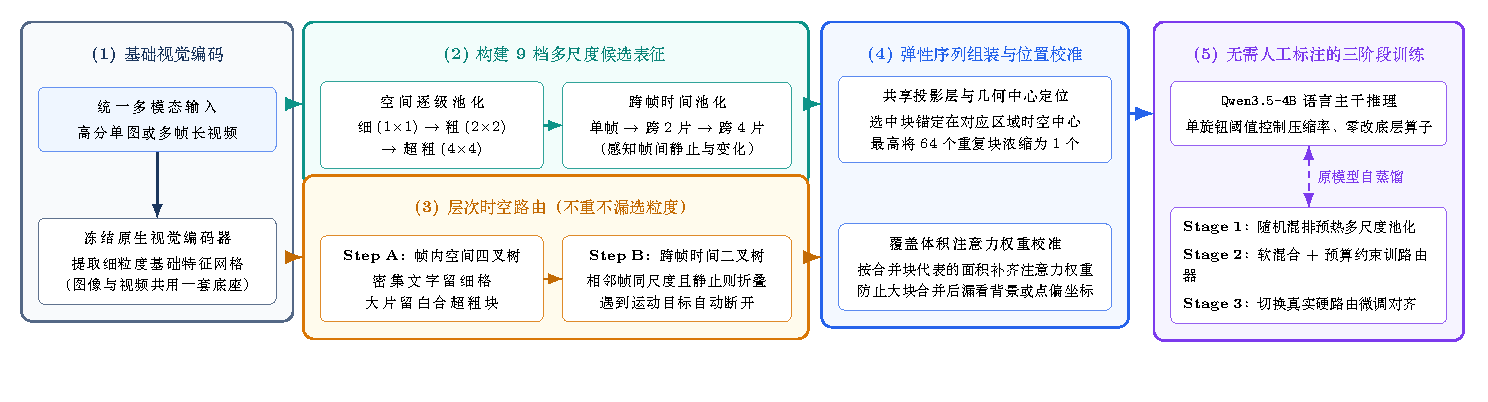
\includegraphics[width=\linewidth]{fig2_method.pdf}
\caption{\textbf{TreeWeave 整体工作流程}：基于冻结视觉编码器提取的细粒度特征，一面通过级联池化准备 9 档时空表征，一面由路由器按``先空间四叉树、后跨帧二叉树''选出最省流的无盲区组合，经中心定位与体积权重校准后送入语言主干，并通过三阶段自蒸馏完成训练。}
\label{fig:method-overview}
\end{figure}

\subsection{\texorpdfstring{核心表征设计：用``空间四叉树 $\times$ 时间二叉树''构建 9 种弹性粒度}{核心表征设计：用空间四叉树 x 时间二叉树构建 9 种弹性粒度}}

为什么不直接用三维图形学里常见的刚性八叉树（每次把长、宽、时间同时各缩一半）？因为刚性绑定有两个明显短板：\textbf{一是单图失效}（单张图片只有 1 帧，无法做时间折半，直接退化回 75\% 压缩上限）；\textbf{二是防不住``静止密集小字''}（视频里的 PPT 或固定字幕在空间上必须保细粒度看清字迹，在时间上却连续多帧不动理应合并）。

因此，我们将空间粗细与时间长短彻底拆开：空间轴设\textbf{细（$1{\times}1$）、粗（$2{\times}2$）、超粗（$4{\times}4$）}三档，时间轴设\textbf{单帧、跨 2 片、跨 4 片}三档，两两正交组合成 \textbf{9 种弹性粒度}（表~\ref{tab:granularities}）。输入单张图像时自动使用左列三档空间四叉树（留白区最高省 \textbf{93.8\%}）；输入视频时全表 9 档按内容激活（静止背景最高 $64{\to}1$ 省 \textbf{98.4\%}，静止小字 $4{\to}1$ 无损省 \textbf{75\%}）。

\begin{table}[H]
\centering
\footnotesize
\setlength{\tabcolsep}{6pt}
\caption{TreeWeave 的 9 种正交时空粒度、Token 浓缩倍率与典型适用区域。}
\label{tab:granularities}
\begin{tabularx}{\linewidth}{@{}l c c c >{\raggedright\arraybackslash}X@{}}
\toprule
\textbf{空间档位 $\backslash$ 时间档位} & \textbf{单帧（不跨帧）} & \textbf{跨 2 片折叠} & \textbf{跨 4 片折叠} & \textbf{最擅长处理的真实画面区域} \\
\midrule
\textbf{细粒度（$1{\times}1$）} & $1{\to}1$（省 0\%） & $2{\to}1$（省 50.0\%） & \cellcolor{AmberSoft}$4{\to}1$（\textbf{省 75.0\%}） & 运动小物体、变化字幕；\textbf{连续静止的 PPT 密集小字/固定 UI 栏} \\
\textbf{粗粒度（$2{\times}2$）} & $4{\to}1$（省 75.0\%） & $8{\to}1$（省 87.5\%） & $16{\to}1$（省 93.8\%） & 普通纹理物体、大号标题文字、缓慢移动的中景 \\
\textbf{超粗粒度（$4{\times}4$）} & \cellcolor{TealSoft}$16{\to}1$（\textbf{省 93.8\%}） & $32{\to}1$（省 96.9\%） & \cellcolor{TealSoft}$64{\to}1$（\textbf{省 98.4\%}） & \textbf{单图文档大片留白/纯色桌面}；\textbf{视频中静止不动的纯色墙面/天空} \\
\bottomrule
\end{tabularx}
\end{table}

\subsection{第一步（怎么造特征）：级联池化生成同一语义空间的候选表征}

我们在冻结的原生视觉编码器（ViT）之上挂载两组极轻量的门控池化模块（总计算量不到视觉编码器的 1\%）：
\begin{itemize}[leftmargin=1.5em, itemsep=3pt]
  \item \textbf{空间逐级池化}：在单帧内部依次将相邻 $2{\times}2$ 区域自适应聚合成``粗粒度''特征，再将相邻 $2{\times}2$ 个粗块聚合成``超粗粒度''特征；
  \item \textbf{感知帧差的时间池化}：在视频相邻帧之间结合帧间特征差异做门控聚合，把连续静止的区域平滑浓缩成跨 2 片或跨 4 片的摘要特征；
  \item \textbf{共用原生投影层}：所有 9 档特征最终都穿过原模型同一套视觉-语言投影层（Merger），保证无论粗细，吐给大语言模型的 Token 都处在完全一致的语义空间里。
\end{itemize}

\subsection{第二步（怎么选粒度）：先空间、后时间的层次树路由与位置校准}

为了保证选出来的粗细块严丝合缝地拼满整张图或整段视频（既不漏掉任何角落，也不重复覆盖），路由器按两步树规则做决策，并配合两项轻量对齐机制：
\begin{enumerate}[leftmargin=1.6em, itemsep=4pt]
  \item \textbf{先做帧内空间四叉树切分}：路由器综合浅层边缘细节与深层语义信息评估每个局部的复杂程度——文字与关键按钮保留细网格，普通区域合并成粗块，只有当一整片 $4{\times}4$ 区域的四个象限全都足够简单（如纯白页边距）时，才整体合并为 1 个超粗大块。单张图片走到这一步即完成编织。
  \item \textbf{再做``同尺度才合并''的跨帧折叠}：对于视频输入，路由器进一步检查相邻帧的同一位置——\textbf{只有当相邻帧在该位置选了相同的空间粗细、且画面几乎没有运动变化时}，才把它们沿时间轴折叠成一个 Token。一旦下一帧有运动目标走入（空间自动切回细粒度），时间折叠就在这一帧边界处干脆断开，从根源上避免动态模糊与拖影。
  \item \textbf{几何中心定位与覆盖体积校准}：任何合并后的粗块，其三维位置编码都精确锚定在它所覆盖区域的时空几何中心；同时，一个合并了 16 格或 64 格的大块在注意力计算中会按其覆盖面积补充相应权重，防止模型``忽略大片背景''或在 GUI 点击任务上算偏坐标。在线部署时，只需调节一个全局阈值旋钮，就能在不重训模型的情况下自由控制省流比例。
\end{enumerate}

\subsection{第三步（怎么训练）：无需人工标注的三阶段自蒸馏}

整个训练过程不需要任何人工标注``哪里该粗、哪里该细''。我们直接拿冻结的原生全细粒度 \texttt{Qwen3.5-4B} 当老师（提前离线跑一遍生成高质量回答并全程复用），分三个职责清晰的阶段训练学生模型（表~\ref{tab:three-stage}）：

\begin{table}[H]
\centering
\footnotesize
\setlength{\tabcolsep}{6pt}
\caption{TreeWeave 三阶段无标注自蒸馏训练流程（每一步只解决一个核心问题）。}
\label{tab:three-stage}
\begin{tabularx}{\linewidth}{@{}l p{3.1cm} >{\raggedright\arraybackslash}X@{}}
\toprule
\textbf{训练阶段} & \textbf{训练哪些模块} & \textbf{具体做法与阶段目的} \\
\midrule
\textbf{Stage 1：预热多尺度池化} & 仅训练空间/时间池化模块与体积校准权重 & 暂不启用路由器，每次随机把画面切成不同粗细组合喂给模型去对齐原模型输出，先把全部 9 档特征池化器练扎实，并让模型提前适应粗细块混排。 \\
\textbf{Stage 2：训练层次路由器} & 冻结主干，仅训练层次时空路由器 & 将离散的``选粗还是选细''松弛为平滑加权混合，在对齐原模型输出的同时加上 Token 数量惩罚与防坍缩约束，端到端逼着路由器学会``在文字和运动处留细格、在留白和静止处省算力''。 \\
\textbf{Stage 3：真实硬路由对齐} & 固定路由器，整体轻量微调池化层与语言模型 & 校准好目标压缩率阈值后，切换回推理时真正使用的离散变长序列做一轮短程微调，彻底消除Stage 2 软混合与线上硬切换之间的细微差距。 \\
\bottomrule
\end{tabularx}
\end{table}

% ======================================================================
\section{实验与消融设计（Experiments \& Ablations on \texttt{Qwen3.5-4B}）}

整个实验章节严格围绕\textbf{``证明 Storyline 中的每一条核心声明''}组织，以 \texttt{Qwen3.5-4B} 作为首发验证基座，在完全对齐的数据与评测协议下展开。

\subsection{核心声明与实验证据映射表（Claim-to-Evidence Map）}

\begin{claimbox}[审稿人视角：每一组实验到底证明什么？]
\begin{itemize}[leftmargin=1.4em, itemsep=3pt]
  \item \textbf{声明 1（突破单图留白上限 + 消除视频帧间冗余）} $\longrightarrow$ \textbf{主实验表 1（8 大基准自适应省流对比）}：直接对比 VisionWeave，证明在同等精度下，文档/GUI 节省率翻倍、视频节省率跃升至 70\%+。
  \item \textbf{声明 2（更高压缩率能换来更高任务能力天花板）} $\longrightarrow$ \textbf{主实验 2（长视频等预算扩帧 \& 多分辨率曲线）}：固定总 Token 预算，TreeWeave 能塞入 $2{\times}{\sim}4{\times}$ 帧数，在长视频基准上显著反超原生模型。
  \item \textbf{声明 3（单模型推理期弹性可控且真实加速服务）} $\longrightarrow$ \textbf{主实验 3（单旋钮阈值帕累托曲线 \& SGLang 实测）}：不重训模型平滑覆盖 0\%--85\%+ 节省区间，并转化为真实的吞吐与延迟收益。
  \item \textbf{声明 4（正交树、学习式路由、体积校准缺一不可）} $\longrightarrow$ \textbf{五大问题驱动消融实验（Ablation Q1--Q5）}。
\end{itemize}
\end{claimbox}

\subsection{主实验方案与 \texttt{Qwen3.5-4B} 对标大表设计}

\paragraph{实验设置（Setup）：}
在 \texttt{Qwen3.5-4B} 上对齐 512 tokens/图（或每视频帧）的标准输入预算，评测覆盖四大领域的 \textbf{8 个代表性基准}：自然图像（RealWorldQA）、密集文档与图表（DocVQA、InfoVQA）、GUI 视觉定位（ScreenSpotV2）、幻觉评测（HallusionBench）、视频文字细节（VideoOCR）以及通用/长视频理解（Video-MME、LongVideoBench）。对比基线涵盖：\textbf{(1)} 原生全 Token 模型（Native）；\textbf{(2)} 固定省 50\% Token 的输入下采样、FastV$^\dagger$（剪枝）、VisionZip（合并）；\textbf{(3)} 最核心直接对手 \textbf{VisionWeave}（表~\ref{tab:main-plan} 已填入其论文公开的 \texttt{Qwen3.5-4B} 精确结果）。

\begin{table}[H]
\centering
\caption{\textbf{主实验大表设计（\texttt{Qwen3.5-4B}）}：前五列为已发表实测基线，最右两列为我们待跑出的核心结果位（重点观察红字标注的 VisionWeave 低节省率痛点任务）。}
\label{tab:main-plan}
\resizebox{\linewidth}{!}{%
\begin{tabular}{@{}l c ccc cc cc@{}}
\toprule
& \textbf{Native} & \multicolumn{3}{c}{\textbf{固定预算基线（Savings = 50\%）}} & \multicolumn{2}{c}{\textbf{VisionWeave（最相近工作）}} & \multicolumn{2}{c}{\cellcolor{SkySoft}\textbf{TreeWeave（本文）}} \\
\cmidrule(lr){2-2}\cmidrule(lr){3-5}\cmidrule(lr){6-7}\cmidrule(l){8-9}
\textbf{Benchmark (\texttt{Qwen3.5-4B})} & Score $\uparrow$ & Downsample & FastV$^\dagger$ & VisionZip & Score $\uparrow$ & Savings $\uparrow$ & \cellcolor{SkySoft}Score $\uparrow$ & \cellcolor{SkySoft}Savings $\uparrow$ \\
\midrule
RealWorldQA（自然场景） & 74.64 & 72.16 & 70.98 & 70.72 & 73.46 & 43.2\% & \cellcolor{SkySoft}\TODO & \cellcolor{SkySoft}\TODO \\
DocVQA（文档 + 页边留白） & 91.92 & 82.71 & 78.69 & 76.57 & 91.03 & \textcolor{Crimson}{\textbf{16.0\%}} & \cellcolor{SkySoft}\TODO & \cellcolor{SkySoft}\TODO \\
InfoVQA（信息海报图表） & 67.44 & 52.87 & 51.75 & 50.89 & 66.11 & \textcolor{Crimson}{\textbf{10.6\%}} & \cellcolor{SkySoft}\TODO & \cellcolor{SkySoft}\TODO \\
ScreenSpotV2（GUI 点击定位） & 89.86 & 80.42 & 72.56 & 70.44 & 89.47 & \textcolor{Crimson}{\textbf{24.1\%}} & \cellcolor{SkySoft}\TODO & \cellcolor{SkySoft}\TODO \\
HallusionBench（抗幻觉） & 69.88 & 69.09 & 69.26 & 68.64 & 69.26 & 44.0\% & \cellcolor{SkySoft}\TODO & \cellcolor{SkySoft}\TODO \\
VideoOCR（视频静态/动态文字） & 64.51 & 59.74 & 63.90 & 63.18 & 63.79 & \textcolor{AmberBorder}{\textbf{47.0\%}} & \cellcolor{SkySoft}\TODO & \cellcolor{SkySoft}\TODO \\
Video-MME（通用视频） & 67.78 & 67.07 & 67.70 & 67.74 & 67.22 & \textcolor{AmberBorder}{\textbf{51.4\%}} & \cellcolor{SkySoft}\TODO & \cellcolor{SkySoft}\TODO \\
LongVideoBench（长视频） & 59.99 & 58.86 & 60.06 & 59.61 & 60.36 & \textcolor{AmberBorder}{\textbf{49.8\%}} & \cellcolor{SkySoft}\TODO & \cellcolor{SkySoft}\TODO \\
\midrule
\rowcolor{RowGray}
\textbf{Average（8 榜均值）} & \textbf{73.25} & 67.87 & 66.86 & 65.97 & \textbf{72.59} & \textbf{35.8\%} & \cellcolor{SkySoft}\textbf{\TODO} & \cellcolor{SkySoft}\textbf{\TODO} \\
\bottomrule
\end{tabular}%
}
\end{table}

\paragraph{除主表外的三组关键主实验图（Result Figures）：}
\begin{enumerate}[leftmargin=1.6em, itemsep=3pt]
  \item \textbf{同等 Token 匹配公平对比（Matched-Budget Comparison）}：把 TreeWeave 在每个数据集上自动测出的高节省率（例如省 60\%--75\%）原样赋予 FastV$^\dagger$、VisionZip 和下采样，证明在高压缩区剪枝基线早已严重崩盘，而 TreeWeave 依然稳住原生精度。
  \item \textbf{长视频``省空间换时间''扩帧实验（Long-Video Frame Scaling）}：在 LongVideoBench 上扫描最大帧数预算（64 $\to$ 128 $\to$ 256 $\to$ 512 帧），画出``总视觉 Token 数 vs.\ 准确率''曲线——直接展示用同样多的视觉 Token，TreeWeave 能看 4 倍长的视频帧，准确率显著超越原生 128 帧上限。
  \item \textbf{推理期单旋钮帕累托曲线与实际部署吞吐}：调节路由阈值画出连续的精度-节省率曲线（直观呈现 VisionWeave 在 75\% 处撞墙截断，而 TreeWeave 平滑延伸至 85\%+），并附上 SGLang 端到端吞吐（req/min）与 TTFT/TPOT 加速表。
\end{enumerate}

\subsection{五大核心消融实验计划（Question-Driven Ablation Study）}

好的消融实验不堆砌无关超参，而是\textbf{每一组消融精准回答审稿人最关心的一个设计追问}（表~\ref{tab:ablations}）：

\begin{table}[H]
\centering
\footnotesize
\setlength{\tabcolsep}{5pt}
\caption{\texttt{Qwen3.5-4B} 上的五组核心消融实验设计（每组严格只变一个因素，对应验证一条方法主张）。}
\label{tab:ablations}
\begin{tabularx}{\linewidth}{@{}p{3.5cm} p{4.2cm} >{\raggedright\arraybackslash}X@{}}
\toprule
\textbf{审稿人核心追问} & \textbf{消融变体设置（Variants）} & \textbf{重点观测指标与预期现象} \\
\midrule
\textbf{Q1：更深的空间层级与跨帧折叠各自带来了多少收益？} &
(a) 仅 2D 两档（退化版 VisionWeave）\newline
(b) 升级为三层空间四叉树（无跨帧）\newline
(c) \textbf{完整正交时空树（TreeWeave）} &
对比 (a)$\to$(b) 在 DocVQA / ScreenSpotV2 上留白区节省率的显著提升；对比 (b)$\to$(c) 在三大视频榜上节省率从 $\sim 55\%$ 向 $75\%+$ 的二次跃升。 \\[4pt]
\textbf{Q2：为什么要做``空间$\otimes$时间正交解耦''，而不是普通 3D 八叉树？} &
(a) \textbf{刚性八叉树变体}（规定空间不粗化的细粒度块禁止跨帧折叠）\newline
(b) \textbf{本文正交解耦树}（允许细空间+粗时间） &
重点在 \textbf{VideoOCR}（含大量连续多帧静止字幕/投屏文字）上对比：刚性八叉树要么省不下 Token，要么强行空间粗化导致文字识别掉点；正交树兼得高压缩与高 OCR 精度。 \\[4pt]
\textbf{Q3：路由器真的学会了按语义密度分配，还是仅仅靠减量？} &
(a) 图内/窗口内\textbf{随机打乱路由（Shuffled）}\newline
(b) 仅用图像像素熵/帧差分的规则启发式路由\newline
(c) \textbf{本文端到端学习路由器} &
严格锁定每条样本完全相同的各档位 Token 数量：验证随机打乱和低层启发式规则在 GUI 定位与密集文档上显著掉点，证明``分给谁''比``留多少''更关键。 \\[4pt]
\textbf{Q4：大跨度合并（$16{\to}1, 64{\to}1$）后为什么空间定位不漂移？} &
(a) 去掉注意力体积校准偏置（w/o Volume Bias）\newline
(b) \textbf{保留注意力体积校准偏置（Ours）} &
重点观测 \textbf{ScreenSpotV2}（GUI 精确坐标预测）在 Stage 2 直接硬路由与 Stage 3 后的准确率差距，验证体积权重补偿对保护空间感知的关键作用。 \\[4pt]
\textbf{Q5：三阶段自蒸馏每个阶段是否都必要？} &
对比 Stage 1 随机多尺度预热 vs.\ 单一尺度预热；对比有无 Stage 3 硬路由微调（及冻结 LLM 轻量变体） &
展示 Stage 1 多尺度预热对超粗档位表征质量的提升，以及 Stage 3 对消除软硬路由间隙的作用。 \\
\bottomrule
\end{tabularx}
\end{table}

\subsection{定性可视化分析规划（Qualitative Case Studies）}
正文最后放一组一锤定音的可视化对比图（直接呼应开篇 Motivation）：
\begin{itemize}[leftmargin=1.5em, itemsep=3pt]
  \item \textbf{案例一（高分辨率财报 / 4K 桌面 GUI）}：并排对比 FastV（删掉关键按钮/残缺文字）、VisionWeave（留白处密密麻麻铺满 $2{\times}2$ 粗块）、\textbf{TreeWeave}（文字按钮处保留细网格、过渡区用粗块、大片留白直接合并为超粗大块，一目了然解释为何省流翻倍且定位不丢）。
  \item \textbf{案例二（网课演讲 / 街景驾驶视频片段）}：展示连续 4 帧切片——运动人物/车辆保持逐帧细网格，静止背景墙合并为跨帧超粗块，而\textbf{静止不动的 PPT 小字区域被精准标为``细空间 + 跨帧折叠''高亮框}，直观印证正交时空树的核心洞察。
\end{itemize}

\end{document}
